\chapter{Análise Exploratória dos Dados e Análise com Modelos de Aprendizado de Máquina}

\section{Distribuição das classes}

Durante nossa análise exploratória, o primeiro passo foi verificar a distribuição da ocorrência das classes no conjunto de dados. Ao calcularmos a distribuição das classes (Figura \ref{fig:distribuicao_classes}) constatamos uma grande desproporção entre as classes. Por exemplo, apenas a classe 'exposed\_soil' representa quase a metade de todo o conjunto de dados. A abundância de exemplos dessas classes majoritárias ('exposed\_soil', 'soybean', 'natural\_vegetation', e etc) pode inundar as classes minoritárias ('eucalyptus', 'grass', 'beans', e etc). A maioria dos algoritmos de aprendizado de máquina para classificação são projetados e demonstrados em problemas que assumem uma distribuição igual de classes. Isso significa que uma aplicação de um modelo pode focar em aprender apenas as características das observações abundantes, negligenciando os exemplos das classes minoritárias.

\begin{figure}[H]
\caption{Distribuição da ocorrência das classes em todo o conjunto de dados.}
\label{fig:distribuicao_classes}
\centering
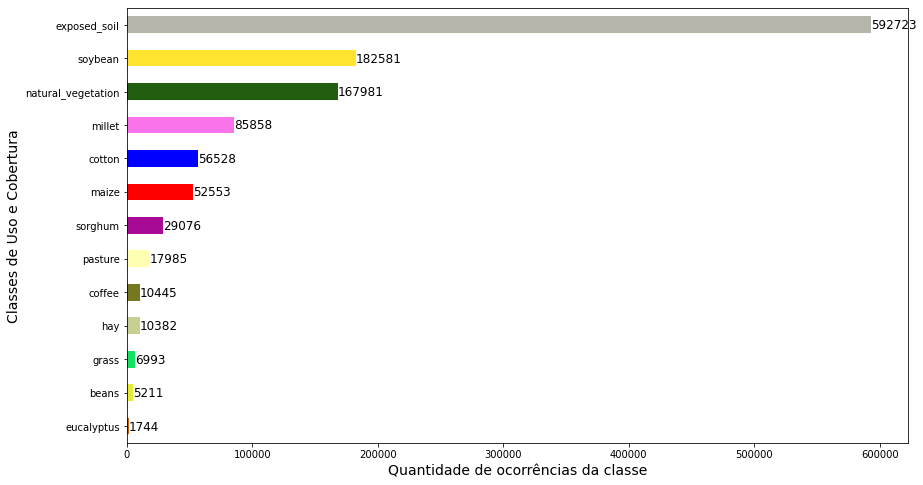
\includegraphics[width=0.6\textwidth]{figuras/ocorrencia_das_classes.png}
\end{figure}


\section{Visualização das \textit{features} nas séries temporais}

Após analisarmos a proporção das classes no conjunto de dados, o próximo passo foi visualizar o comportamento das \textit{features} nas séries temporais. Ao analisar as \textit{features} nas séries temporais, é possível identificarmos o comportamento que cada \textit{feature} tem com a mudança da classe de uso e cobertura. Por exemplo, na Figura \ref{fig:features_na_serie_temporal} é possível identificarmos que na classe 'soybean', a \textit{feature} 'RED' tende a ter valores menores e a \textit{feature} 'NIR' tende a ter valores maiores, em comparação com a classe 'exposed\_soil'. Também é possível identificarmos que a \textit{feature} 'NDVI', gerada a partir das diferença normalizada das \textit{features} 'NIR' e 'RED' tente a ter valores mais altos na classe 'soybean' do que na classe 'exposed\_soil', o que indica que essa \textit{feature} pode ser usada pelo algoritmos para diferenciar essas duas classes.

\begin{figure}[H]
\caption{Exemplo de uma série temporal com as \textit{features} utilizadas para o treinamento dos modelos e suas classes de uso e cobertura da terra correspondentes ao longo do tempo.}
\label{fig:features_na_serie_temporal}
\centering
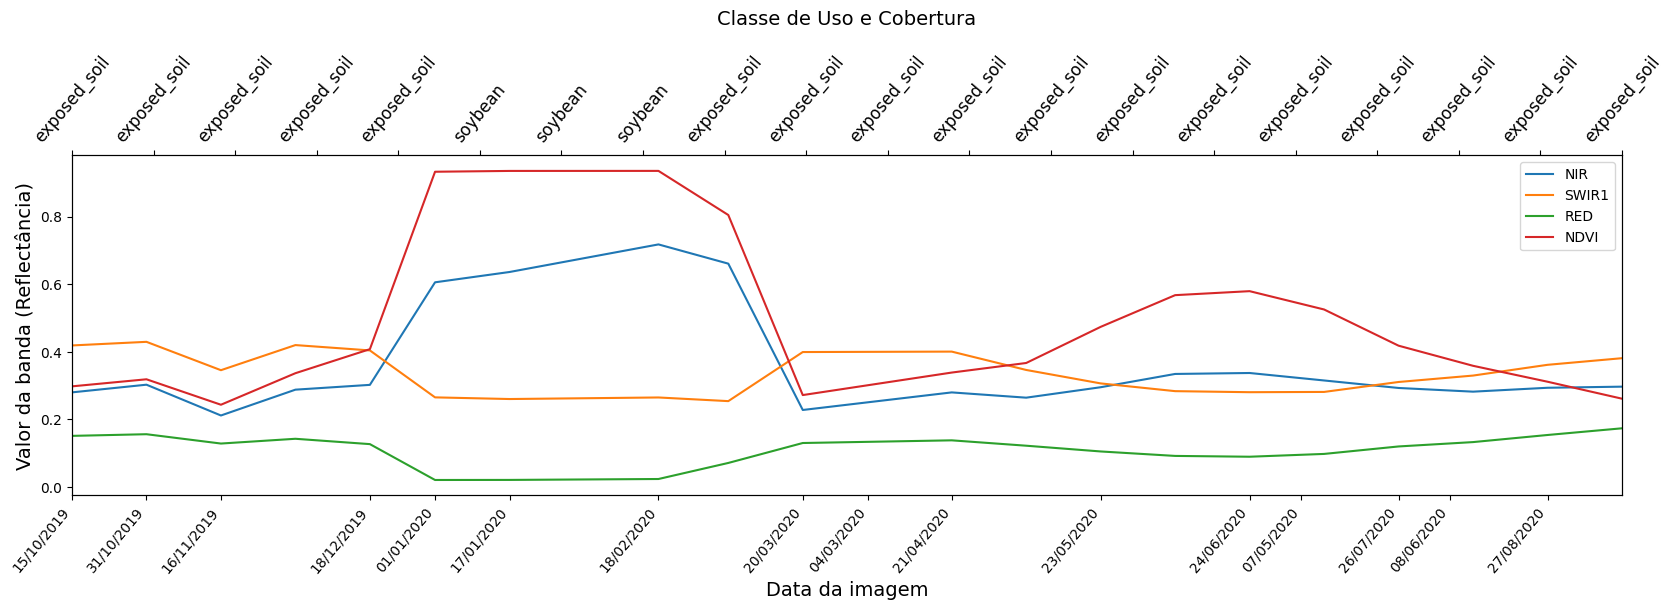
\includegraphics[width=0.8\textwidth]{figuras/serie_temporal_features.png}
\end{figure}

\section{Análise de valores discrepantes nas séries temporais}

Valores discrepantes são valores que diferem significativamente dos padrões e tendências dos outros valores do conjunto de dados. Na geração das séries temporais, utilizamos como referência a classe indicada pelo analista para o respectivo mês daquele produto de imagem de satélite. Como para um único mês temos sempre dois produtos de imagens de satélite, é possível que o analista tenha, por exemplo, indicado que no mês da análise a classe de uso seja um cultivo de soja, porém nas imagens de satélite aquela soja seja visível apenas no primeiro produto do mês, já no segundo produto, após uma eventual colheita no meio do mês, esse produto pode ter sido indicado como cultivo de soja ('soybean'), mas essa área já tenha ficado com o comportamento espectral de solo exposto ('exposed\_soil') após a colheita. Na Figura \ref{fig:boxplot_das_features_com_outliers} é possível identificarmos, através da análise dos diagramas de caixa, que muitas das classes apresentam valores discrepantes. No caso da classe de soja ('soybean'), por exemplo, é esperado que os valores do 'NDVI' fiquem acima de 0,4 \cite{risso2009potencialidade}, porém nos diagramas é possível observarmos que existem observações indicadas como soja com valores de 'NDVI' abaixo de 0,4, indicando, possivelmente, que essas áreas já foram colhidas. 

Para evitarmos que esses valores discrepantes interfiram negativamente nos modelos criados, realizamos a remoção de todas essas observações discrepantes em todas as classes mapeadas. Antes da remoção dos valores discrepantes, haviam 1.523.364 observações em todo o conjunto de dados, após a eliminação dos valores discrepantes restaram 1.384.317 observações, ou seja, uma eliminação de quase 10\% de valores discrepantes.

\begin{figure}[H]
\caption{Distribuição dos valores, por classe de uso e cobertura, das observações em cada uma das \textit{features} utilizadas para treinar os modelos. Nos diagramas, os valores discrepantes não foram removidos.}
\label{fig:boxplot_das_features_com_outliers}
\centering
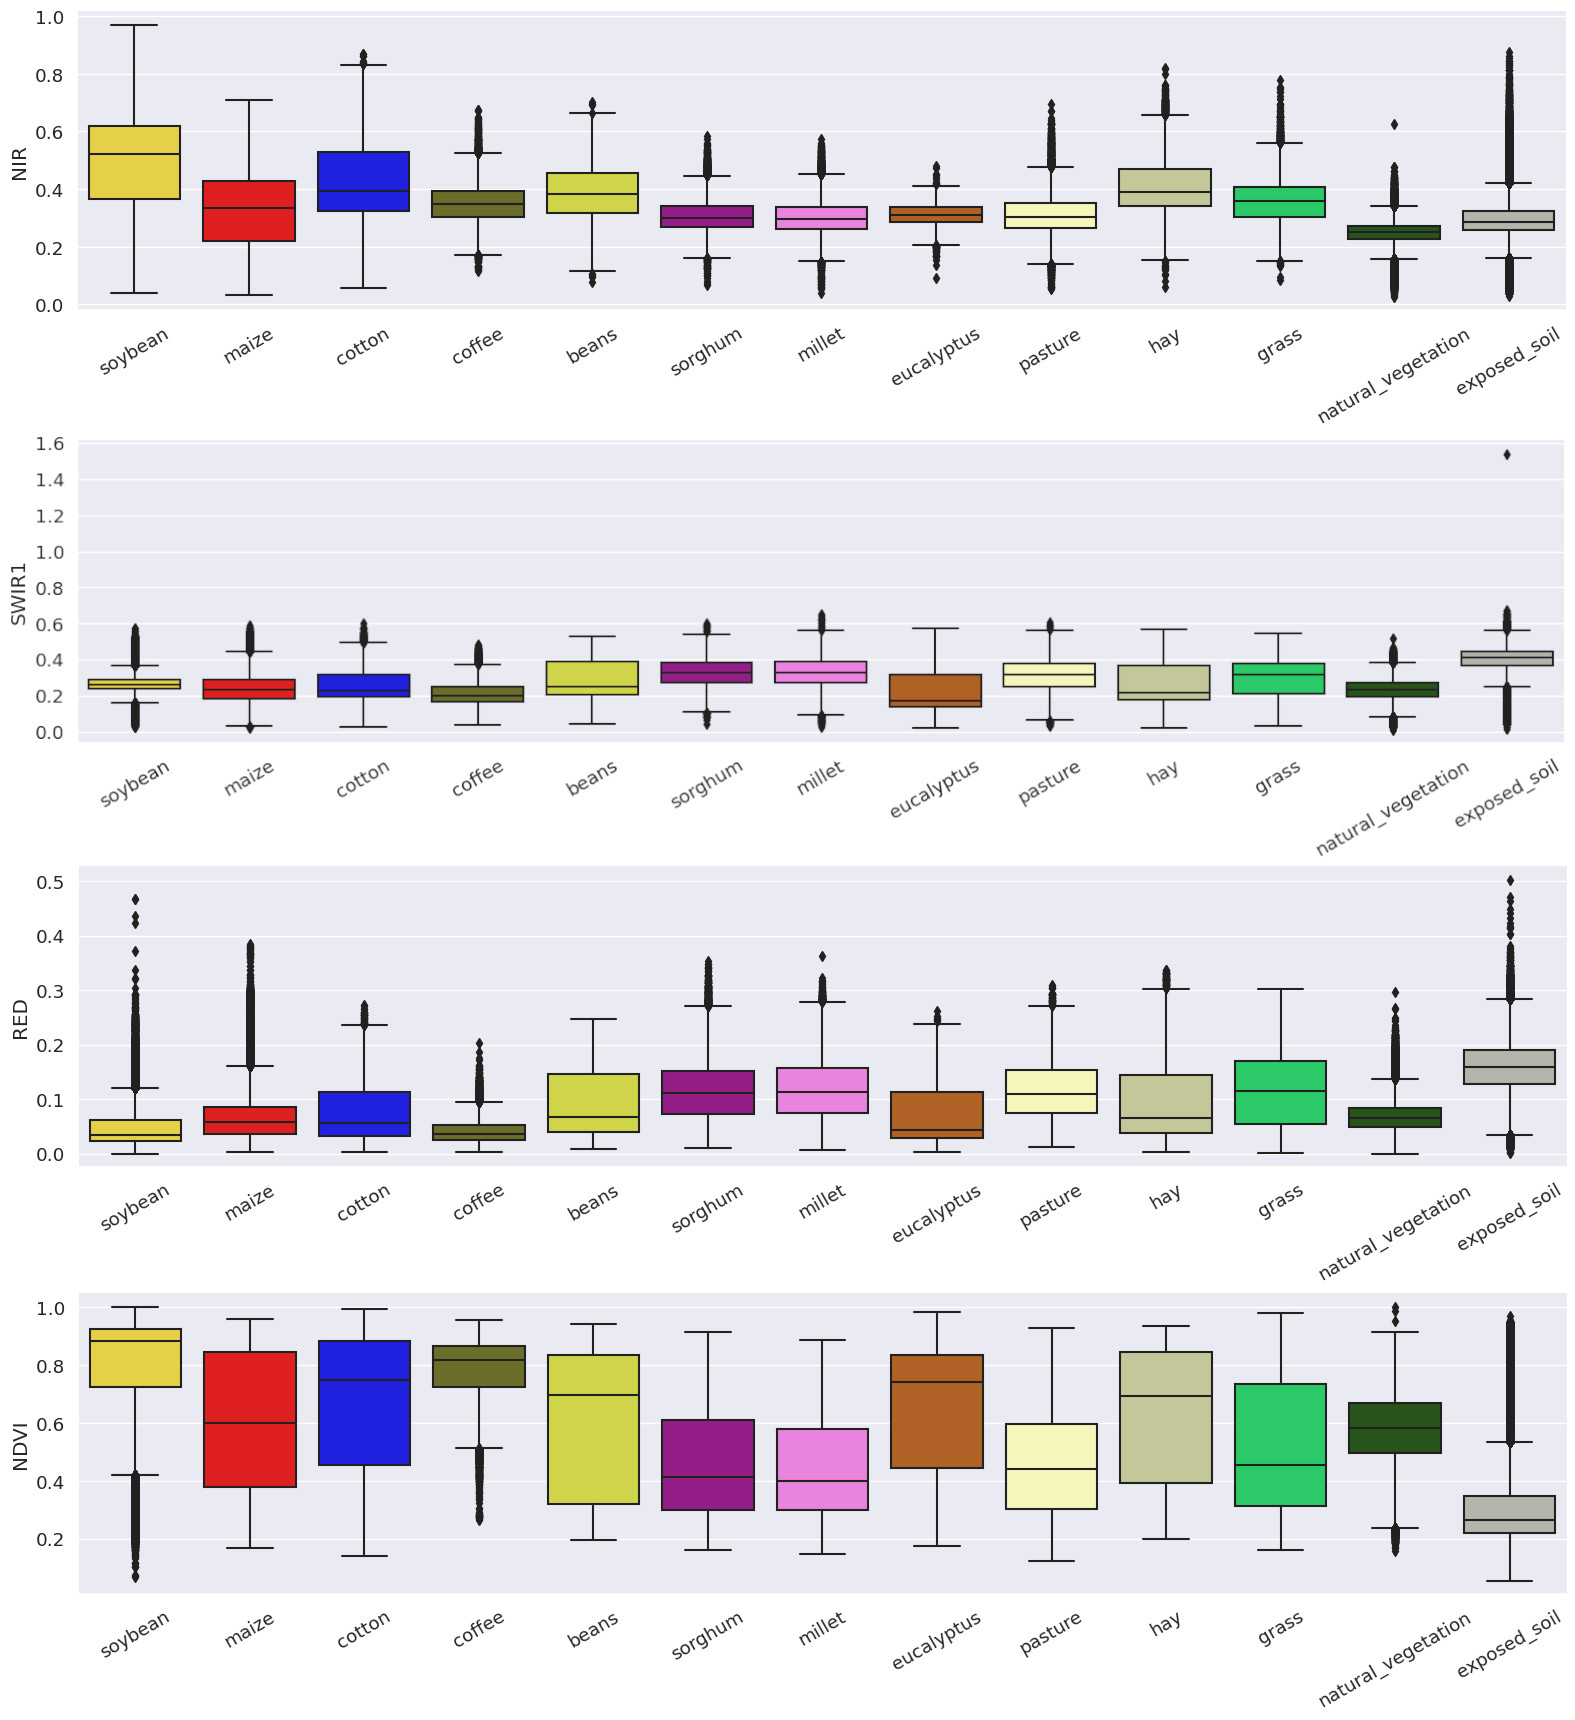
\includegraphics[width=0.6\textwidth]{figuras/catplot_features.jpg}
\end{figure}

\section{Análise da capacidade das \textit{features} em separar as classes de uso e cobertura da terra que foram mapeadas}

Após a eliminação das observações discrepantes, a próxima análise que executamos foi verificar a capacidade de cada uma das \textit{features} de separar determinadas classes de uso e cobertura. Na Figura \ref{fig:analise_confusao_entre_classes_por_feature} é possível verificarmos quais \textit{features} melhor contribuiem para a separação de determinadas classes. Por exemplo, é possível observarmos que as \textit{features} 'RED' e 'NDVI' melhor contribuem para a separação entre as classes 'soybean', 'exposed\_soil' e 'natural\_vegetation'. Nos gráficos é possível observar que, nessas \textit{features}, essas classes possuem uma menor sobreposição entre as curvas, o que indica que um modelo de aprendizado de máquina terá maior facilidade em separar essas classes com essas \textit{features}. Ainda na Figura \ref{fig:analise_confusao_entre_classes_por_feature}, é possível analisarmos se a combinação de duas \textit{features} pode ajudar a separar determinadas classes. Por exemplo, Na combinação entre as \textit{features} ('NIR', 'RED'), ('SWIR1', 'RED'), ('SWIR1', 'NIR'), ('NDVI', 'NIR') e ('NDVI', 'SWIR1) é possível observarmos que os pontos da classe 'soybean' ficam mais agrupados e separados dos demais do que nas outras combinações, o que pode indicar que a combinação dessas \textit{features} pode auxiliar na identificação dessa classe. 

\begin{figure}[H]
\caption{Gráficos com a distribuição dos valores, por classe, para combinações entre as diferentes \textit{features} (gráficos de pontos) e entre a mesma \textit{feature} (gráficos de linhas).}
\label{fig:analise_confusao_entre_classes_por_feature}
\centering
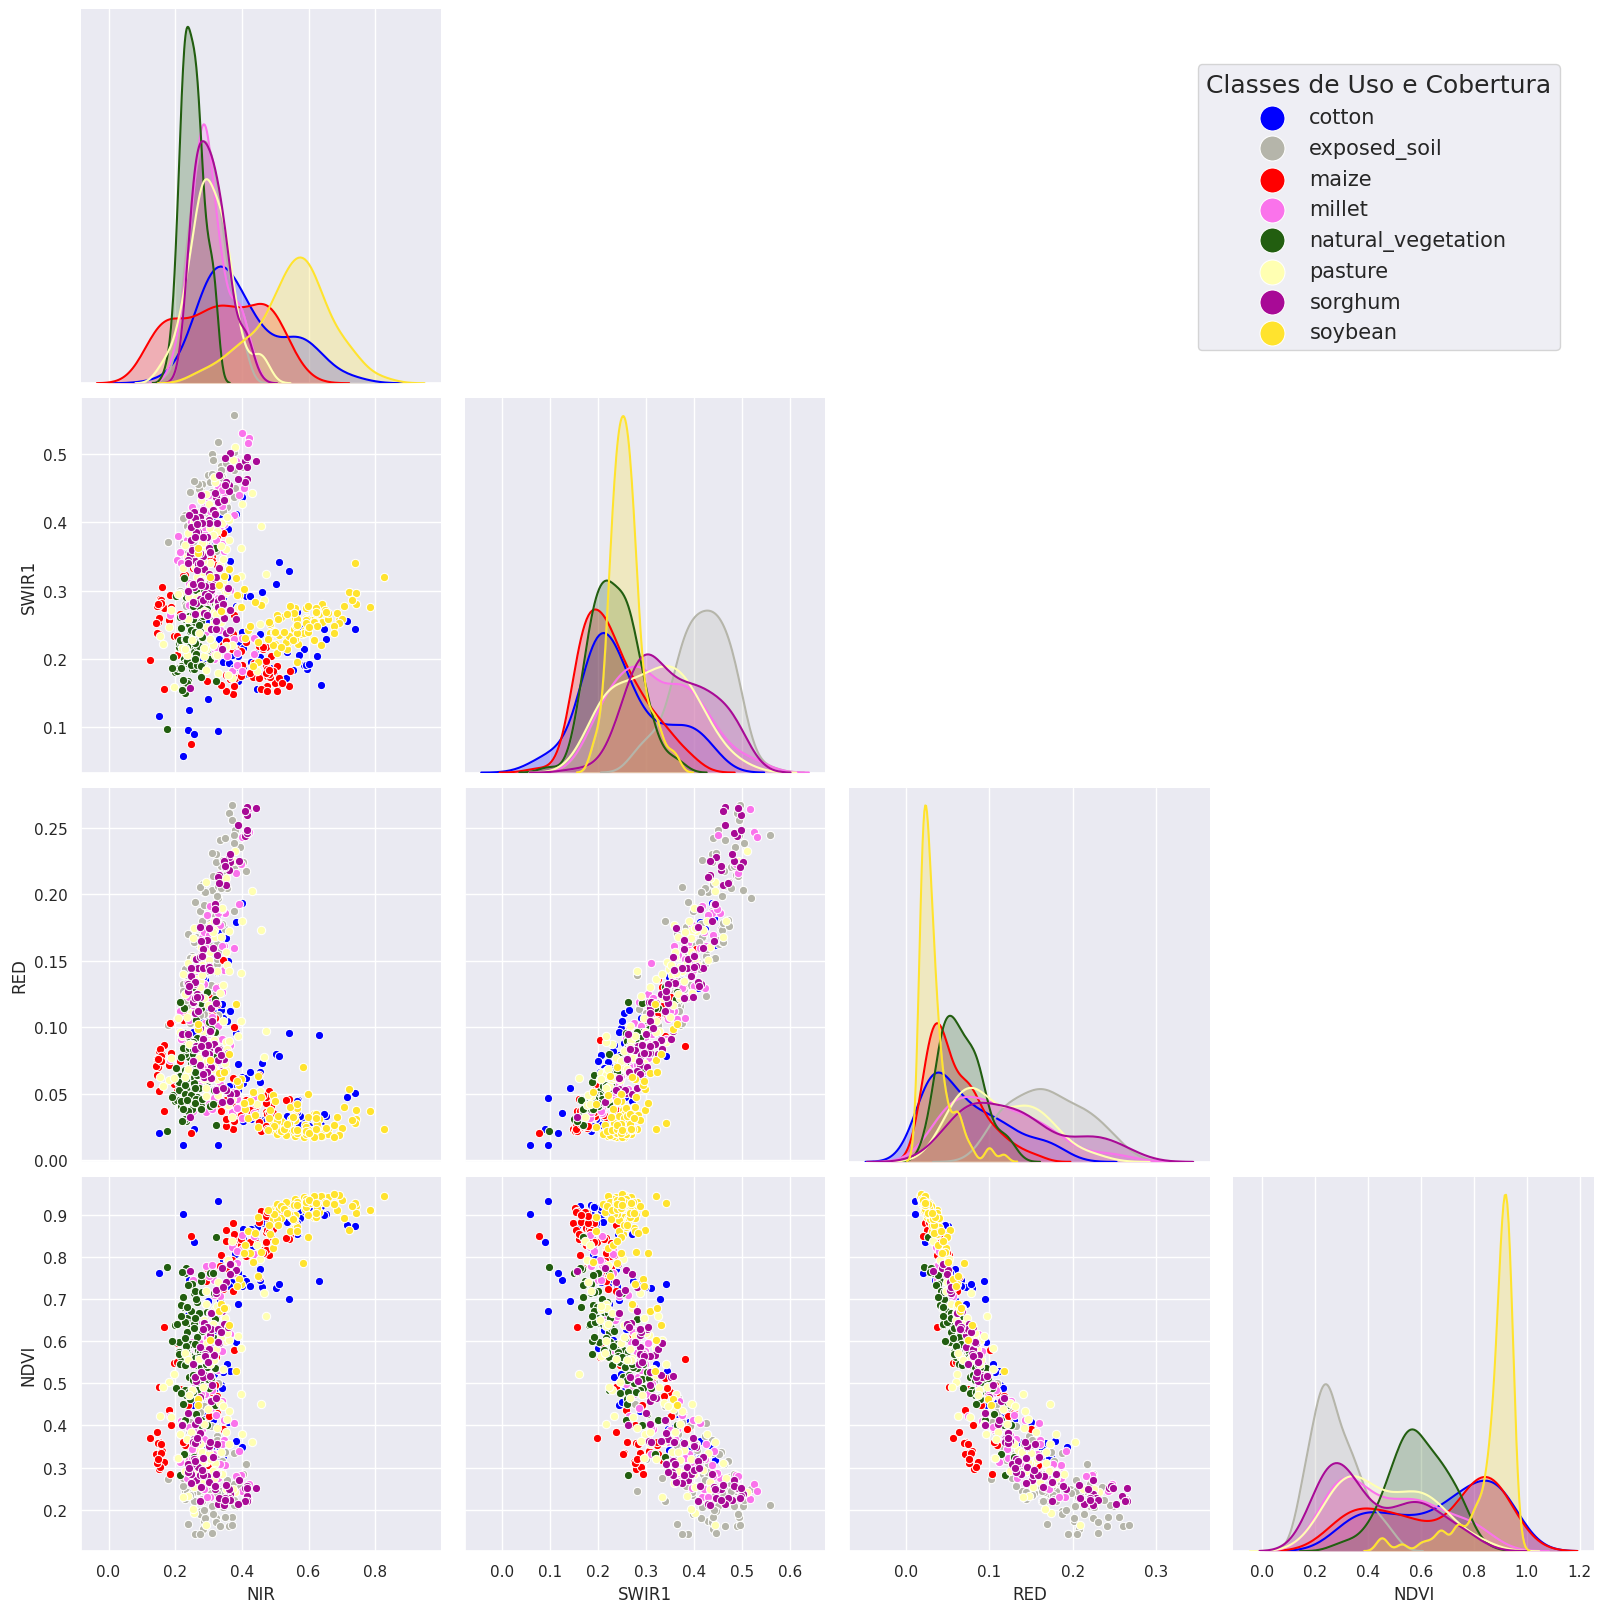
\includegraphics[width=0.5\textwidth]{figuras/correlacao_features_por_classe.png}
\end{figure}

\section{Criação dos modelos de Aprendizado de Máquina}

Neste trabalho, avaliamos três modelos de classificação de uso e cobertura da terra, dois modelos baseado em árvores de decisão utilizando Random Forest \cite{breiman2001random} e um modelo baseado em redes neurais recorrentes utilizando a arquitetura Long Short-Term Memory (LSTM) \cite{hochreiter1997long}.


O Random Forest é um dos algoritmos mais populares para classificação supervisionada  das últimas décadas, sua popularidade é devido, principalmente, às seus ótimos resultados obtidos sem muita parametrização e sem muita necessidade de um grande conjunto de dados de treinamento. 

Rede Neural Recorrente (RNN) é um tipo de Rede Neural onde a saída da etapa anterior é alimentada como entrada para a etapa atual, ou seja, ela possui uma “memória” que guarda todas as informações sobre o que foi calculado. A arquitetura de RNN que utilizamos foi a chamada Long Short-Term Memory - LSTM, uma arquitetura de rede neural recorrente específica que foi projetada para modelar sequências temporais e suas dependências de longo alcance com mais precisão do que RNNs convencionais \cite{sak2014long}, característica importante quando trabalhamos com séries temporais mais longas. 

Para o treinamento e análise da acurácia dos modelos, os dados foram separados em três conjuntos distintos: 80\% treinamento, 10\% validação e 10\% teste. Segundo \citeonline{hastie2009elements}, o conjunto de treinamento deve ser usado para ajustar o modelo; o conjunto de validação deve ser usado para estimar o erro da predição do modelo, e o conjunto de teste deve ser utilizado para a avaliação do erro da generalização do modelo final escolhido. 


\subsection{Modelo Random Forest}

Para a classificação utilizando o Random Forest, utilizamos duas diferentes bibliotecas. A primeira foi a biblioteca scikit-learn, versão 0.24.2, que implementa o Random Forest classico através da classe RandomForestClassifier. Já a segunda foi a biblioteca imbalanced-learn, versão 0.8.1, que implementa uma versão adaptada do Random Forest através da classe BalancedRandomForestClassifier, que aplica um balanceamento entres as classes para dar maior importância as classes minoritárias durante o processo de treinamento do modelo (Figura \ref{fig:parametros_random_forest}). 

\begin{figure}[H]
\centering
\caption{Parâmetros utilizados nos classificadores baseados em Random Forest com e sem o balanceamento das classes.}
\label{fig:parametros_random_forest}
\begin{lstlisting}[language=Python]
# Importando as classes
from sklearn.ensemble import RandomForestClassifier
from imblearn.ensemble import BalancedRandomForestClassifier

# Random Forest sem balanceamento das classes
rf_model = RandomForestClassifier(n_estimators=200, random_state=1, n_jobs=-1)

# Random Forest com balanceamento das classes
brf_model = BalancedRandomForestClassifier(n_estimators=200, random_state=1, n_jobs=-1)

\end{lstlisting}
\end{figure}

\subsection{Modelo LSTM}

Para a construção do modelo LSTM, utilizamos a biblioteca TensorFlow, versão 2.3.0. O modelo que desenvolvemos (Figura \ref{fig:arquitetura_lstm}) utiliza duas camadas LSTM com 128 neurônios cada. Para camada de saída utilizamos uma camada do tipo TimeDistributed com uma camada densamente conectada com a quantidade de neurônios igual a quantidade de classes que queremos mapear. Para ativação da última camada utilizamos a função Softmax. Essa combinação na camada de saída faz com que a saída do modelo seja, para cada ponto da série temporal, uma lista com as probabilidades para cada classe.  Configuramos o modelo para utilizar o otimizador \textit{Adam}, função de perda \textit{categorical\_crossentropy} e como métrica de avaliação a \textit{categorical\_accuracy}, todos parâmetros disponíveis na biblioteca TensorFlow. 

\begin{figure}[H]
\centering
\caption{Arquitetura baseada em LSTM utilizada para a classificação das séries temporais.}
\label{fig:arquitetura_lstm}
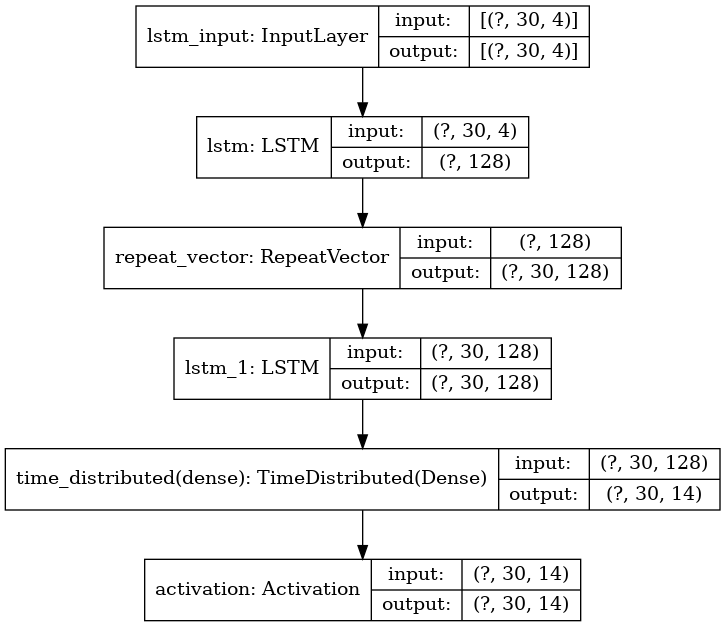
\includegraphics[width=0.4\textwidth]{figuras/lstm.png}
\end{figure}

\renewcommand{\cleardoublepage}{}
\renewcommand{\clearpage}{}
\vspace{5mm}